%   ####
%
%   Band VIII, 3 N.~??A13
%   Signatur/Tex-Datei: LH_35_09_15_021
%   RK-Nr. 41156
%   Überschrift: [De chordarum tensione (ex: De chordarum vibrationibus)]
%   Datierung: [Ende Dezember 1680 oder Anfang 1681; (?) Sommer 1682 bis ??März/April 1683]
%   WZ: 8-blättrige Rosette über CS (RK-WZ: 138)
%.  SZ: (keins)
%.  Bilddateien (PDF): LH_35_09_15_021_d1; LH_35_09_15_021_d2; LH_35_09_15_021_d3; LH_35_09_15_021_d4; LH_35_09_15_021_d5 (insgesamt fünf)
%
%
\begin{ledgroupsized}[r]{120mm}
\footnotesize
\pstart
\noindent
\textbf{Überlieferung:}
\pend
\end{ledgroupsized}
\begin{ledgroupsized}[r]{114mm}
\footnotesize
\pstart \parindent -6mm
\makebox[6mm][l]{\textit{L}}%
Aufzeichnung: LH~XXXV~9,~15 Bl.~21.
Ein Blatt~4\textsuperscript{o};
Fragment eines Wasserzeichens.
Anderthalb Seiten, tlw. einspaltig beschrieben.
% Zahlreiche Streichungen, Ergänzungen und Ersetzungen.
Am Ende von Bl.~21~r\textsuperscript{o} weist ein Kustos auf den Anfang von Bl.~21~v\textsuperscript{o} hin.
Die Schlussbemerkung
(S.~\refpassage{LH_35_09_15_021v_schluss-1}{LH_35_09_15_021v_schluss-2})
ist wohl % von Leibniz 
nachträglich hinzugefügt worden.
\pend
\end{ledgroupsized}
%
%
\vspace{5mm}
\begin{ledgroup}
\footnotesize
\pstart
\noindent
\textbf{Datierungsgründe:}
Das vorliegende Stück N.~10, das auf für Leibnizens erste Hannoveraner Zeit mehr\-fach belegtem Papier verfasst ist, weist einen engen inhaltlichen Zusammenhang mit N.~8 \textit{Tentaminum de chordarum tensione schedae} (Dezember 1680) auf.
Dies zeigt sich auch daran, dass in N.~10 % \textendash\ 
ebenso wie in N.~8 % \textendash\ 
das Verhältnis zwischen der Dicke einer % gespannten 
Saite und der Frequenz ihrer Schwingung noch der Vorlage entspricht, die Leibniz in H.~Fabris\protect\index{Namensregister}{\textso{Fabri}, Honoré 1607\textendash1688} \cite{00044}\textit{Physica} vorfand
(vgl. N.~10, S.~\refpassage{LH_35_09_15_021r_crassitiessuperflua-1}{LH_35_09_15_021r_crassitiessuperflua-2} mit 
N.~8\textsubscript{2}, S.~\refpassage{LH_35_09_15_009v_crassitiessuperflua-1}{LH_35_09_15_009v_crassitiessuperflua-2}; 
N.~8\textsubscript{4}, S.~\refpassage{LH_35_09_15_012v_crassitiessuperflua-1}{LH_35_09_15_012v_crassitiessuperflua-2}; 
N.~8\textsubscript{6}, S.~\refpassage{LH_35_09_15_016r_crassitiessuperflua-1}{LH_35_09_15_016r_crassitiessuperflua-2}).
Dem Ansatz nach knüpft N.~10 vornehmlich an N.~8\textsubscript{6} an:
Möglicherweise hätte N.~10 die (nicht weiter ermittelten) Untersuchungen über den Isochronismus der Schwingungen umfassen sollen, die u.a. am Ende von N.~8\textsubscript{6} (S.~\refpassage{LH_35_09_15_017v_Schluss_rfas-1}{LH_35_09_15_017v_Schluss_rfas-2}) angekündigt werden.
Demnach dürfte N.~10 etwa zur gleichen Zeit wie N.~8\textsubscript{6} (10./20. Dezember 1680) oder etwas später entstanden sein.
\pend%
\pstart%
Die\edlabel{LH_35_09_15_021v_schlussbemerkung-1} am Ende von N.~10 mit anderer Tinte verfasste Bemerkung (S.~\refpassage{LH_35_09_15_021v_schluss-1}{LH_35_09_15_021v_schluss-2}) muss jedoch nach\-träglich hinzugefügt worden sein.
Leibniz spielt dort offenbar auf die Überlegungen zur Bruchfestigkeit der Balken 
an, die er ab Ende Juli/Anfang August 1682 im Austausch mit E.~Mariotte\protect\index{Namensregister}{\textso{Mariotte}, Edme, Seigneur de Chazeuil ca. 1620\textendash1684} entwickelte und
in dem zwischen Ende Januar 1683 und Ende Juni 1684 entstandenen Textkomplex N.~14 niederschrieb (siehe die editorische Vorbemerkung hierzu, S.~\pageref{AE_1684_319-325_intro_jecg}\,ff.).
Dort unterscheidet er zwei Betrachtungsweisen bzw. \glqq Hypothesen\grqq\ über den Bruch eines Balkens:
Die eine, die er Galilei\protect\index{Namensregister}{\textso{Galilei} (Galilaeus, Galileus), Galileo 1564\textendash1642} zuschreibt, geht von der Annahme eines vollkommen starren, auf einmal durchbrechenden Balkens aus (vgl. tatsächlich G.\,\textsc{Galilei}, \textit{Discorsi}, Leiden 1638, S.~114\,f.\cite{00050}; \textit{GO} VIII, S.~156\,f.\cite{00048});
die andere \glqq Hypothese\grqq, von Mariotte und Leibniz selbst vertreten, setzt hingegen einen bis zum Bruch stetig biegsamen Balken voraus (siehe etwa N.~14\textsubscript{6}, S.~\refpassage{LH_35_09_15_021v_duaehypotheseis-1}{LH_35_09_15_021v_duaehypotheseis-2}; \refpassage{LH_35_09_15_021v_duaehypotheseis-3}{LH_35_09_15_021v_duaehypotheseis-4}; dieselbe Unterscheidung liegt aber bereits N.~14\textsubscript{1} zugrunde).
Aus diesen verschiedenen Grundannahmen folgen verschiedene Berechnungen des Bruchwiderstands eines Balkens (siehe die editorische Vorbemerkung zu N.~14, S.~\refpassage{AE_1684_319-325_intro_LeibizAnMariotte-1}{AE_1684_319-325_intro_LeibizAnMariotte-2}).
Nur nach Leibnizens \glqq Hypothese\grqq\ gilt aber, dass der Balken entlang der Bruchlinie einen Widerstand leistet, der in einem quadratischen Verhältnis zum Abstand vom Bruchzentrum steht (N.~14\textsubscript{6}, S.~\refpassage{LH_35_09_15_021v_Verweis_Quadrat-1}{LH_35_09_15_021v_Verweis_Quadrat-2});
nach der Galilei zugeschriebenen \glqq Hypothese\grqq\ soll dieses Verhältnis vielmehr linear sein (ebd., S.~\refpassage{LH_35_09_15_021v_HypothGalilei-1}{LH_35_09_15_021v_HypothGalilei-2}).
Somit ist nicht unmittelbar ersichtlich, worauf Leibniz genau anspielt, wenn er in der Schlussbemerkung von N.~10 festhält: \textit{diversas licet proportiones tamen rem reducere demum ad duplicatam, ut in resistentia solidorum expertus sum, sive Galilei\protect\index{Namensregister}{\textso{Galilei} (Galilaeus, Galileus), Galileo 1564\textendash1642} hypothesi sive mea uterer} (S.~\refpassage{LH_35_09_15_021v_schluss-1}{LH_35_09_15_021v_schluss-2}).
Trotzdem ist nicht zu bestreiten, dass diese Beobachtung auf die Auseinandersetzung mit der Festigkeit der Balken im Rahmen des Textkomplexes N.~14 anspielt.
Daher kann die Schlussbemerkung nur nach Ende Juli/Anfang August 1682 verfasst worden sein.
Da Leibniz aber ab März/April 1683 aufhört, Galileis \glqq Hypothese\grqq\ als gleichberechtigte Betrachtungsweise zu behandeln (siehe die editorische Vorbemerkung zu N.~14, S.~\refpassage{AE_1684_319-325_intro_Brief456_pwyu-1}{AE_1684_319-325_intro_Brief456_pwyu-2}), so dürfte die Schlussbemerkung noch davor entstanden sein.%
\edlabel{LH_35_09_15_021v_schlussbemerkung-2}
\pend
\end{ledgroup}
%
%
 \newpage%
%\vspace{8mm}%
\pstart%
\normalsize%
\noindent%
%
\lbrack21~r\textsuperscript{o}\rbrack\ % Blatt 21 r
%
\pend%
%
%  \newpage
  \vspace{1.0em}%
  \centerline{\hspace*{-4mm}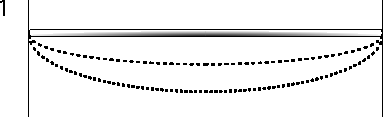
\includegraphics[width=0.40\textwidth]{gesamttex/edit_VIII,3/images/LH_35_09_15_021_d1.pdf}}%
  \vspace{0.5em}%
  \centerline{\lbrack\textit{Fig.~1}\rbrack}%
  \vspace{1.5em}%
%
\pstart%
\noindent%
(1)\edlabel{LH_35_09_15_021r_propositio1-1}
Unius chordae\protect\index{Sachverzeichnis}{chorda tensa}
(\phantom)\hspace*{-1.2mm}%
eandem longitudinem\protect\index{Sachverzeichnis}{longitudo chordae}
et tensionem\protect\index{Sachverzeichnis}{tensio chordae} servantis%
\phantom(\hspace*{-1.2mm})
vibrationes\protect\index{Sachverzeichnis}{vibratio chordae}
majores minoresque sunt aequediuturnae.%
\edlabel{LH_35_09_15_021r_propositio1-2}\protect\index{Sachverzeichnis}{vibratio aequidiuturna}
\pend%
%
%  \newpage
  \vspace{1.5em}%
  \centerline{\hspace*{-4,6mm}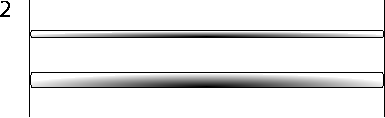
\includegraphics[width=0.40\textwidth]{gesamttex/edit_VIII,3/images/LH_35_09_15_021_d2.pdf}}%
  \vspace{0.5em}%
  \centerline{\lbrack\textit{Fig.~2}\rbrack}%
  \vspace{1.5em}%
%   \newpage
%
\pstart%
\noindent%
(2)
\edlabel{LH_35_09_15_021r_crassitiessuperflua-1}%
Duae chordae ejusdem materiae\protect\index{Sachverzeichnis}{materia chordae}
uniformis\protect\index{Sachverzeichnis}{materia uniformis}
\edtext{quae sunt}{%
\lemma{quae}\Bfootnote{%
\hspace{-0,5mm}sunt
\textit{erg.~L}}}
aeque tensae\protect\index{Sachverzeichnis}{chorda tensa}
\edtext{et}{%
\lemma{et}\Bfootnote{\textit{erg.~L}}}
aeque longae,
\edtext{sed inaequaliter crassae}{%
\lemma{sed inaequaliter crassae}\Cfootnote{%
Siehe \cite{00044}H.~\textsc{Fabri}, \textit{Physica}, tract.~III, lib.~II, prop.~223; 224
(Bd.~II, Lyon 1670, S.~215b; 216a; 216b).}}%
\lbrack,\rbrack\
%
nihilominus habent tempora vibrationum\protect\index{Sachverzeichnis}{tempus vibrationis}
aequalia\lbrack,\rbrack
\edlabel{LH_35_09_15_021r_crassitiessuperflua-2}
\edtext{nisi aeris resistentia\protect\index{Sachverzeichnis}{resistentia aeris} obstet.
Forte tamen non obstat.}{%
\lemma{nisi}\Bfootnote{%
\hspace{-0,5mm}aeris \lbrack...\rbrack\ non obstat
\textit{erg.~L}}}
\pend%
%
%  \newpage
  \vspace{1.5em}%
  \centerline{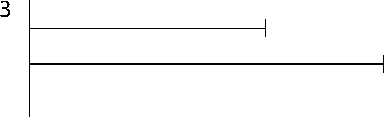
\includegraphics[width=0.40\textwidth]{gesamttex/edit_VIII,3/images/LH_35_09_15_021_d3.pdf}}%
  \vspace{0.5em}
  \centerline{\lbrack\textit{Fig.~3}\rbrack}%
  %
   \vspace{1.5em}
  \pstart%
\noindent%
(3) Duae chorde aeque tensae,\protect\index{Sachverzeichnis}{chorda tensa}
sed longitudine inaequales
habent tempora vibrationum\protect\index{Sachverzeichnis}{tempus vibrationis}
in ratione longitudinum.\edlabel{LH_35_09_15_021r_Abs3-1}%
\protect\index{Sachverzeichnis}{longitudo chordae}%
\edtext{}{{\xxref{LH_35_09_15_021r_Abs3-1}{LH_35_09_15_021r_Abs3-2}}{%
\lemma{longitudinum.}\Bfootnote{%
\hspace{-0,5mm}\textbar~(4) \textit{gestr.}~%
\textbar\ Unius%
~\textit{L}}}}
\pend%
%\vspace{0.5em}
\newpage
  \centerline{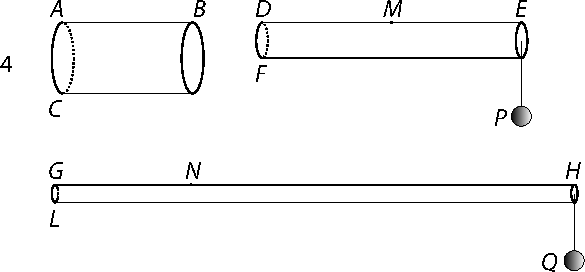
\includegraphics[width=0.62\textwidth]{gesamttex/edit_VIII,3/images/LH_35_09_15_021_d4.pdf}}%
  \vspace{0.5em}
  \centerline{\lbrack\textit{Fig.~4}\rbrack}%
%  \edtext{}{\lemma{\lbrack\textit{Fig.~4}\rbrack}\killnumber\Cfootnote{**************************}}
  \vspace{1.5em}%
%
\count\Bfootins=1200
\count\Afootins=1200
\count\Cfootins=1200
%
 \pstart%
\noindent%
Unius\edlabel{LH_35_09_15_021r_Abs3-2}
ejusdemque chordae\protect\index{Sachverzeichnis}{chorda tensa}
\edtext{tensiones\protect\index{Sachverzeichnis}{tensio chordae} seu vires
quibus in unaquaque tensione sustentari potest,\protect\index{Sachverzeichnis}{vis tendens}
sunt ut quantitates excessuum\protect\index{Sachverzeichnis}{quantitas excessus}}{%
\lemma{tensiones}\Bfootnote{%
\textit{(1)}~sunt inter se
\textit{(2)}~seu vires quibus in
\textit{(a)}~ea tensione
\textit{(b)}~unaquaque tensione \lbrack...\rbrack\ sunt ut
\textit{(aa)}~longitudines. $\langle$Ad hanc jam positionem$\rangle$
\textit{(bb)}~quantitates excessuum%
~\textit{L}}}
super statum\protect\index{Sachverzeichnis}{status chordae}
\edtext{naturalem.\protect\index{Sachverzeichnis}{status naturalis}
Quae ut aestimentur considerandum est chordam}{%
\lemma{naturalem.}\Bfootnote{%
\textit{(1)}~Nam
\textit{(2)}~Quae ut aestimentur
\textit{(a)}~consideranda
\textit{(b)}~considerandum est
\textit{(aa)}~chorda
\textit{(bb)}~chordam%
~\textit{L}}}
eo magis tensam\protect\index{Sachverzeichnis}{chorda tensa} esse
quo fit tenuior,
\edtext{seu spatium\protect\index{Sachverzeichnis}{spatium chordae} occupat angustius,}{%
\lemma{seu}\Bfootnote{%
\textit{(1)}~minus
\textit{(2)}~spatium occupat angustius,%
~\textit{L}}}
quo autem spatium occupat angustius,
eo necesse est ut longior sit.
Sit chorda cujus status\protect\index{Sachverzeichnis}{status chordae}
naturalis\protect\index{Sachverzeichnis}{status naturalis} \textit{ABC},
violenti\protect\index{Sachverzeichnis}{status violentus}
duo \textit{DEF} et \textit{GHL},
sitque basis\protect\index{Sachverzeichnis}{basis chordae}
seu circulus\protect\index{Sachverzeichnis}{circulus} \textit{DF},
dimidius baseos seu circuli \textit{AC},
\edtext{erit \textit{DE} dupla}{%
\lemma{erit}\Bfootnote{%
\textit{(1)}~\textit{GH} dim
\textit{(2)}~\textit{DE}
\textit{(a)}~dimidia
\textit{(b)}~dupla%
~\textit{L}}}
\edtext{ipsius}{%
\lemma{ipsius}\Bfootnote{\textit{erg.~L}}}
\textit{AB}.
Si vero basis\protect\index{Sachverzeichnis}{basis chordae}
seu circulus \textit{GL} sit quarta pars
circuli\protect\index{Sachverzeichnis}{circulus} \textit{AC},
erit longitudo\protect\index{Sachverzeichnis}{longitudo chordae}
\textit{GH} quadrupla ipsius
\edtext{\textit{AB}.
Certum est}{%
\lemma{\textit{AB}.}\Bfootnote{%
\textit{(1)}~Ajo vires
\textit{(2)}~Sit \textit{DM} aequ. \textit{AB}, et \textit{GN} etiam aequ. \textit{AB}.
Dico tensiones\protect\index{Sachverzeichnis}{tensio chordae}
seu vires tendentes\protect\index{Sachverzeichnis}{vis tendens}
chordam \textit{AB}, in chordam \textit{DE}
\textit{(a)}~vel
\textit{(b)}~et \textit{GH} esse inter se ut \textit{ME} ad \textit{NH}.
Quod sic ostendo.
\textit{(3)}~Certum est%
~\textit{L}}}
vim ad tendendum necessariam\protect\index{Sachverzeichnis}{vis ad tendendum necessaria}
sumendam esse a quantitate effectus.\protect\index{Sachverzeichnis}{quantitas effectus}
Effectus autem totus\protect\index{Sachverzeichnis}{effectus totus}
aestimari potest a chordae tenuitate,\protect\index{Sachverzeichnis}{tenuitas chordae}
nam eo tensior est chorda\protect\index{Sachverzeichnis}{chorda tensa}
quo est tenuior.
Tenuitatem\protect\index{Sachverzeichnis}{tenuitas chordae}
autem aestimo non a diametro,\protect\index{Sachverzeichnis}{diameter chordae}
sed a tota area baseos,\protect\index{Sachverzeichnis}{basis chordae}
\edtext{seu angustia spatii\protect\index{Sachverzeichnis}{angustia spatii} quod occupatur.}{%
\lemma{seu}\Bfootnote{%
\textit{(1)}~spatio quod occupatur
\textit{(2)}~angustia spatii quod occupatur.%
~\textit{L}}}
\count\Bfootins=900
\count\Afootins=1000
\count\Cfootins=900
Est ergo status\protect\index{Sachverzeichnis}{status chordae}
violentus\protect\index{Sachverzeichnis}{status violentus}
excessus tenuitatis,\protect\index{Sachverzeichnis}{excessus tenuitatis}
id est diminutio
\edtext{baseos,\protect\index{Sachverzeichnis}{basis chordae}
seu erit pondus\protect\index{Sachverzeichnis}{pondus tendens}
\textit{P} ad pondus\protect\index{Sachverzeichnis}{pondus tendens} \textit{Q}
ut $\text{circ.}\, AC - \text{circ.}\, DF$ ad $\text{circ.}\, AC - \text{circ.}\, GL.$
Sive:}{%
\lemma{baseos,}\Bfootnote{%
\textit{(1)}~differentia autem inter basin \textit{FD} et \textit{AC} est ad differentiam
\textit{(2)}~jam \textit{AC} :
\textit{(3)}~\textit{DF} et \textit{AC}
\textit{(4)}~seu erit
\textit{(a)}~vis
\textit{(b)}~pondus \textit{P} \lbrack...\rbrack\ circ. \textit{GL}.
\textit{(aa)}~Jam
\textit{(bb)}~Sive:%
~\textit{L}}}
\edtext{$P : Q \,\overset{\wideparen{1}}{\squaredots}\, \astrosun AC - \astrosun DF :
\edtext{\astrosun AC - \astrosun\, GL.$
Jam
$\astrosun AC : \astrosun DF \,\protect\overset{\wideparen{2}}{\squaredots}\, DE : AB.$}{%
\lemma{$\astrosun AC - \astrosun\!\ GL.$}\Bfootnote{%
\textit{(1)}~Jam
\textit{(2)}~Sive $P : Q \ \squaredots$
\textit{(3)}~Jam $\astrosun AC : \astrosun DF \,\protect\overset{\wideparen{2}}{\squaredots}\, DE : AB.$%
~\textit{L}}}
Et
$\astrosun AC : \astrosun GL \,\overset{\wideparen{3}}{\squaredots}\, GH : AB.$
Ergo
$\astrosun DF\protect\rule[-3mm]{0mm}{9mm} \,\overset{\wideparen{4}}{\text{aequ}}.\, \displaystyle\frac{\astrosun AC \cdot AB}{DE}$
et
$\astrosun\, GL \,\overset{\wideparen{5}}{\text{aequ}}.\, \displaystyle\frac{\astrosun AC \cdot AB}{GH}.$
Quos valores\protect\index{Sachverzeichnis}{valor}
$\scriptstyle{4}$, $\scriptstyle{5}$
substituendo in proport. $\scriptstyle{1}$,
fiet:
$\displaystyle P : Q \,\squaredots\,
\astrosun AC - \frac{\astrosun AC \cdot AB}{DE} : \astrosun AC - \frac{\astrosun AC \cdot AB}{GH}$
seu
$\displaystyle \squaredots\, \frac{DE - AB}{DE} :
\edtext{\frac{GH -AB}{GH}.$
Ergo}{%
\lemma{$\displaystyle\frac{GH -AB}{GH}.$}\Bfootnote{%
\textit{(1)}~Seu
\textit{(2)}~Ergo%
~\textit{L}}}%
\protect\rule[-2mm]{0mm}{7mm} $P : Q \,\squaredots\, GH \cdot DE - AB \cdot GH : GH \cdot DE - AB \cdot DE.$%
}{\lemma{$P : Q$ \lbrack...\rbrack\ $AB \cdot DE$\,}\Cfootnote{%
In den Proportionen hat Leibniz bei auftretenden Differenzen die an sich nötigen Klammern vernachlässigt.}}
\pend%
%
\count\Bfootins=900
\count\Afootins=1000
\count\Cfootins=900
\pstart%
Cum tamen contrarius oriturus fuisset calculus\protect\index{Sachverzeichnis}{calculus contrarius}
si non a tenuitate\protect\index{Sachverzeichnis}{tenuitas chordae} incepissemus
indeque ad longitudinem\protect\index{Sachverzeichnis}{longitudo chordae} fuissemus ratiocinati,
sed incepissemus a longitudine\protect\index{Sachverzeichnis}{longitudo chordae}
ratiocinantes inde ad tenuitatem,\protect\index{Sachverzeichnis}{tenuitas chordae}
itaque non est probus hic calculus,\protect\index{Sachverzeichnis}{calculus probus}
sed assumendus ejusmodi
qui utrobique succedat eodem modo,
sive longitudine\protect\index{Sachverzeichnis}{longitudo chordae} sola,
sive tenuitate\protect\index{Sachverzeichnis}{tenuitas chordae} sola rem aestimes.
\pend%
%
\pstart%
Effectus ergo quantitas\protect\index{Sachverzeichnis}{quantitas effectus}
aestimanda a quantitate
\edtext{transmutationis.\protect\index{Sachverzeichnis}{quantitas transmutationis}
Ea vero aestimabitur}{%
\lemma{transmutationis.}\Bfootnote{%
\textit{(1)}~Ea erit
\textit{(2)}~Ea vero aestimabitur%
~\textit{L}}}
ratione ipsius \textit{DE} ad \textit{AB} sive \textit{GH} ad \textit{AB}.
Quo posito
\edtext{erunt vires\protect\index{Sachverzeichnis}{vis tendens}
inter se ut longitudines,\protect\index{Sachverzeichnis}{longitudo chordae}}{%
\lemma{erunt}\Bfootnote{%
\textit{(1)}~inter se ut longitudines
\textit{(2)}~vires inter se ut longitudines,%
~\textit{L}}}
vel ut tenuitates\protect\index{Sachverzeichnis}{tenuitas chordae}
sive reciproce ut bases;\protect\index{Sachverzeichnis}{basis chordae}
sive reciproce ut quadrata diametrorum.\protect\index{Sachverzeichnis}{diameter chordae}
Nimirum non tam spectandum quantum longitudini\protect\index{Sachverzeichnis}{longitudo chordae}
adjectum vel tenuitati\protect\index{Sachverzeichnis}{tenuitas chordae} ademtum;
sed quae sit ratio producti ad prius.%
\pend%
% \newpage%  ! ! ! ! ! Rein vorläufig ! ! ! ! !
%
  \pstart%
 Sane considerandum an chorda jam
\edtext{tensa\protect\index{Sachverzeichnis}{chorda tensa} difficilius}{%
\lemma{tensa}\Bfootnote{%
\hspace{-0,5mm}\textbar~non \textit{gestr.}~%
\textbar\ difficilius%
~\textit{L}}}
tendatur ut
\edtext{ante.
Quod si dicamus
% // unius ejusdemque chordae
%
\lbrack21~v\textsuperscript{o}\rbrack\ % Blatt 21 v
%
unius ejusdemque chordae\protect\index{Sachverzeichnis}{chorda tensa}
vires tendentes\protect\index{Sachverzeichnis}{vis tendens}
seu tensiones\protect\index{Sachverzeichnis}{tensio chordae}
esse ut longitudines,\protect\index{Sachverzeichnis}{longitudo chordae}}{%
\lemma{ante.}\Bfootnote{%
\textit{(1)}~Sed si hoc non est, concludo:
% \textit{(a)}~
(4) Unius ejusdemque chordae tensiones seu vires tendentes esse ut longitudines
\textit{(2)}~Quod si  \lbrack...\rbrack\ ut longitudines,%
~\textit{L}}}
tunc etiam oriri videtur absurdum.\protect\index{Sachverzeichnis}{absurdum}
Nam in statu\protect\index{Sachverzeichnis}{status chordae}
naturali,\protect\index{Sachverzeichnis}{status naturalis}
seu in quo chorda\protect\index{Sachverzeichnis}{chorda tensa} sponte sua manet,
nulla est tensio,\protect\index{Sachverzeichnis}{tensio chordae}
neque vis tendens,\protect\index{Sachverzeichnis}{vis tendens}
et tamen est aliqua longitudo.\protect\index{Sachverzeichnis}{longitudo chordae}
An ergo erunt vires\protect\index{Sachverzeichnis}{vis tendens}
ut logarithmi\protect\index{Sachverzeichnis}{logarithmus} rationum
\edtext{longitudinis\protect\index{Sachverzeichnis}{longitudo chordae}
unius ad alteram\lbrack:\rbrack\
cum nulla longitudo\protect\index{Sachverzeichnis}{longitudo chordae}
una alteri aequalis est,}{%
\lemma{longitudinis}\Bfootnote{%
\textit{(1)}~violentae\protect\index{Sachverzeichnis}{longitudo chordae violenta}
\textbar~ad naturalem\protect\index{Sachverzeichnis}{longitudo chordae naturalis}
\textit{streicht Hrsg.}~\textbar\
\textit{(2)}~unius ad alteram
\textit{(a)}~tunc enim non
\textit{(b)}~cum nulla
\textit{(aa)}~est
\textit{(bb)}~longitudo una alteri aequalis est,%
~\textit{L}}}
seu cum eadem relicta,
\edtext{logarithmus\protect\index{Sachverzeichnis}{logarithmus}
(\phantom)\hspace*{-1.2mm}%
pro unitate\protect\index{Sachverzeichnis}{unitas} scilicet,
seu ratione aequalitatis%
\phantom(\hspace*{-1.2mm}) erit nihil.\protect\index{Sachverzeichnis}{nihil}}{%
\lemma{logarithmus}\Bfootnote{%
\textit{(1)}~erit
\textit{(2)}~(\phantom)\hspace*{-1.2mm}unitatis scilicet
\textit{(3)}~(\phantom)\hspace*{-1.2mm}pro unitate \lbrack...\rbrack\ aequalitatis\phantom(\hspace*{-1.2mm}) erit
\textit{(a)}~unitas
\textit{(b)}~nihil.%
~\textit{L}}}
Verum nobis non licet pro arbitrio\protect\index{Sachverzeichnis}{arbitrium} nostro
\edtext{sic fingere}{%
\lemma{sic}\Bfootnote{%
\textit{(1)}~fingi
\textit{(2)}~fingere%
~\textit{L}}}
proportiones
etsi in aliquibus consentiant.
\pend%
%
%\newpage
%\count\Bfootins=1200
%\count\Afootins=1200
%\count\Cfootins=1200
%   \centerline{\hspace*{-4mm}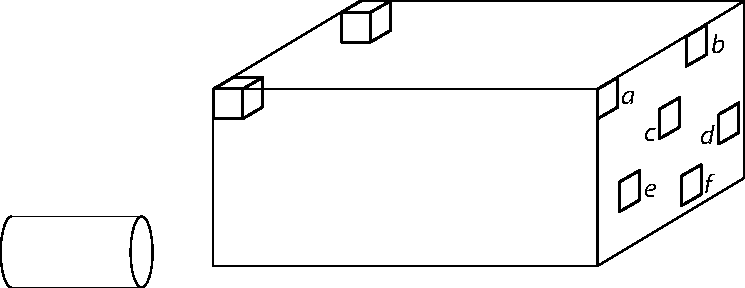
\includegraphics[width=0.66\textwidth]{gesamttex/edit_VIII,3/images/LH_35_09_15_021_d5.pdf}}%
%  \vspace{0.5em}
%  \centerline{\lbrack\textit{Fig.~5}\rbrack}%
%  \vspace{1.5em}%
\pstart%
%\edtext{}{\lemma{%   !  !  !  !   Achtung getrixt: Folgende Afootnote sollte an [Fig. 5] hängen.  !  !  !  !
%\hspace*{1,6mm}\textit{Unter} \lbrack\textit{Fig.~5}\rbrack:}\killnumber\Afootnote{%
%Ponamus Prisma\protect\index{Sachverzeichnis}{prisma}
%constare ex meris quadratillis\protect\index{Sachverzeichnis}{quadratillum}\lbrack,\rbrack\
%horum plurima \textit{a} \textit{b} \textit{c} \textit{d} \textit{f}
%intervallis\protect\index{Sachverzeichnis}{intervallum} dissita
%educi una cum his
%quae post ea sunt per totam prismatis longitudinem\lbrack,\rbrack\
%educta autem in unum compelli.}}
Non licebit ex hac incertitudine\protect\index{Sachverzeichnis}{incertitudo} exire
donec fingamus Machinam\protect\index{Sachverzeichnis}{machina}
ex multis particulis\protect\index{Sachverzeichnis}{particula} compositam,
eamque secundum leges\protect\index{Sachverzeichnis}{lex}
hypotheseos nostrae\protect\index{Sachverzeichnis}{hypothesis nostra}
seu assumtae tensorum naturae\protect\index{Sachverzeichnis}{natura tensi} tractemus.
\pend%
\newpage
 \centerline{\hspace*{-4mm}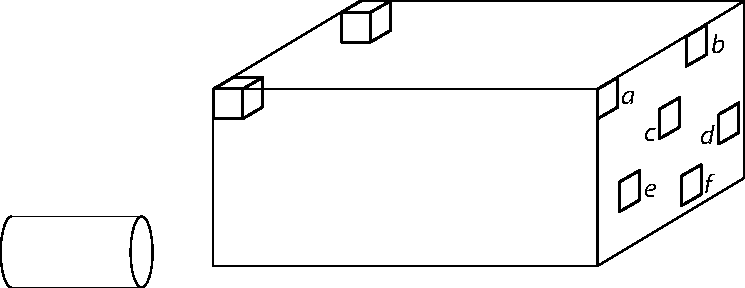
\includegraphics[width=0.66\textwidth]{gesamttex/edit_VIII,3/images/LH_35_09_15_021_d5.pdf}}%
  \vspace{0.5em}
  \centerline{\lbrack\textit{Fig.~5}\rbrack}%
  \vspace{1.5em}
%\newpage 
 \pstart%
%
\edtext{}{%
{\xxref{LH_35_09_15_021v_schluss-1}{LH_35_09_15_021v_schluss-2}}%
{\lemma{Notandum \lbrack...\rbrack\ uterer}\Cfootnote{%
Die Schlussbemerkung ist mit einer anderen Tinte und in einem anderen Schreibduktus verfasst als der übrige Text.}}}%
Notandum\edlabel{LH_35_09_15_021v_schluss-1} est diversas licet proportiones % \lbrack,\rbrack\
tamen rem reducere demum ad duplica\-tam,\protect\index{Sachverzeichnis}{proportio duplicata}
\edtext{ut in resistentia solidorum\protect\index{Sachverzeichnis}{resistentia solidi}
expertus sum, sive
% \edtext{
Galilei\protect\index{Namensregister}{\textso{Galilei} (Galilaeus, Galileus), Galileo 1564\textendash1642}
hypothesi\protect\index{Sachverzeichnis}{hypothesis Galileiana}
sive mea\protect\index{Sachverzeichnis}{hypothesis mea}
% }{%
% \lemma{Galilei \lbrack...\rbrack\ mea}\Cfootnote{%
% Für die Über\-windung der Bruchfestigkeit eines Balkens wird Galileis \glqq Hypothese\grqq\ zufolge die Hälfte der Kraft (Gewicht) benötigt, die für die Überwindung der Zugfestigkeit desselben Balkens erforderlich ist;
% vgl. \textit{Discorsi}, Leiden 1638, S.~114f.\cite{00050} (\textit{GO} VIII, S.~156f.\cite{00048}).
% Leibnizens \glqq Hypothese\grqq\ zufolge wird für die Überwindung der Bruchfestigkeit nur ein Drittel der für die Über\-windung der Zugfestigkeit erforderlichen Kraft benötigt.
% Dieser Berechnungs\-unterschied rührt davon her, dass Leibniz \textendash\ anders als Galilei \textendash\ die Möglichkeit völlig unbiegsamer Körper ausschließt.
% Stattdessen nimmt er an, dass ein Balken sich immer zunächst biegt, wenn er quer abgerissen wird,
% und dass bei dieser Biegung die Bestandteile des Balkens einen Widerstand ent\-lang der Bruchlinie leisten,
% welcher nach dem Quadrat des Abstandes vom Bruchzentrum wächst
% (siehe etwa N.~??20, bes. S.~??163.25\textendash??165.5).}}
% \refpassage{LH_35_09_15_021v_brchfst-1}{LH_35_09_15_021v_brchfst-2}
uterer.\edlabel{LH_35_09_15_021v_schluss-2}%
}{%
\lemma{ut \lbrack...\rbrack\ uterer}\Cfootnote{%
% Die von Leibniz zu Beginn der achtziger Jahre vertretenen Ansichten über die Festigkeit von Körpern (etwa Balken) lassen sich vornehmlich den \textit{Demonstrationes novae de resistentia solidorum} entnehmen.
% Siehe N.~?? und ??19.1.
%
% Es ist nicht ersichtlich, worauf sich diese Feststellung bezieht.
% Die Unterschiede zwischen Leibniz und Galilei bei der Auffassung der Festigkeit werden besonders im ??späteren Aufsatz N.~??A19\textsubscript{1}, S.~\refpassage{LH_35_09_15_021v_brchfst-1}{LH_35_09_15_021v_brchfst-2}.
%
Siehe hierzu die Erläuterung in den Datierungsgründen (S.~\refpassage{LH_35_09_15_021v_schlussbemerkung-1}{LH_35_09_15_021v_schlussbemerkung-2}).
}}%
\edtext{}{\lemma{%   !  !  !  !   Achtung getrixt: Folgende Afootnote sollte an [Fig. 5] hängen.  !  !  !  !
\hspace*{1,6mm}\textit{Unter} \lbrack\textit{Fig.~5}\rbrack:}\killnumber\Afootnote{%
Ponamus Prisma\protect\index{Sachverzeichnis}{prisma}
constare ex meris quadratillis\protect\index{Sachverzeichnis}{quadratillum}\lbrack,\rbrack\
horum plurima \textit{a} \textit{b} \textit{c} \textit{d} \textit{f}
intervallis\protect\index{Sachverzeichnis}{intervallum} dissita
educi una cum his
quae post ea sunt per totam prismatis longitudinem\lbrack,\rbrack\
educta autem in unum compelli.\newline}}%
%
\pend%
\count\Bfootins=1200
\count\Afootins=1200
\count\Cfootins=1200
%
%
% ENDE DES STÜCKES auf Blatt 21v